\documentclass[a4paper,12pt]{article}

\usepackage[utf8]{inputenc}
\usepackage{graphicx}
\usepackage[table]{xcolor}
\usepackage{pdfpages}
\usepackage{hyperref}
\usepackage{float}
\usepackage[top=1in, bottom=1.25in, left=1in, right=1in]{geometry}
\usepackage{wrapfig}
\usepackage{enumitem}
\usepackage{gensymb}
\usepackage{fancyref}
\usepackage{amssymb}
\usepackage{supertabular}

\renewcommand{\familydefault}{\sfdefault}

\definecolor{routinevisualadvisorycolor}{rgb}{0, 1, 0}
\definecolor{nonroutinevisualadvisorycolor}{rgb}{1.0, 0.85, 0}
\definecolor{lightgrey}{rgb}{0.9, 0.9, 0.9}
\definecolor{tablehdrcolor}{rgb}{0.9, 0.9, 1.0}
\definecolor{tablecontcolor}{rgb}{0.95, 0.95, 0.95}
\definecolor{noteboxcolor}{rgb}{.98, 0.8, 0}

\newcommand{\visualadvisory}[3][b]{%
    \ifthenelse{\equal{#1}{b}}{\begin{center}}{}
    \noindent
    \colorbox{black}{\textcolor{#2visualadvisorycolor}{\large\texttt{~#3~}}}
    \ifthenelse{\equal{#1}{b}}{\end{center}}{}}

\newcommand{\filetext}[1]{\vspace{.5em}%
\noindent\hspace{0.05\textwidth}\fcolorbox{black}{lightgrey}{%
\parbox{0.9\textwidth}{\texttt{#1}}}%
\vspace{.5em}}

\newcommand{\notebox}[1]{\vspace{.5em}%
\noindent\hspace{0.05\textwidth}\fcolorbox{black}{noteboxcolor}{%
\parbox{0.9\textwidth}{{\large\bf NOTE}\vspace{.35em}\hrule\vspace{.25em}#1}}%
\vspace{.5em}}

\newcommand{\confopt}[1]{\texttt{#1}}

\newcommand{\myfrac}[2]{%
\textsuperscript{#1}\hspace{-0.4em}$\diagup$\hspace{-0.4em}\textsubscript{#2}}

\newcommand{\fileicon}[1]{\raisebox{-.15em}%
{\includegraphics[height=.9em]{../src/#1}}}

\setlist{nolistsep}

\setlength{\abovecaptionskip}{0pt}
\setlength{\belowcaptionskip}{0pt}
\setlength\intextsep{0pt}

\overfullrule=2cm

\title{X-RAAS 2.0 User Manual}
\author{Sašo Kiselkov}


\begin{document}

\includepdf{../src/cover.pdf}

\tableofcontents

\newpage

\listoffigures

\newpage

\section{Introduction}

X-RAAS implements a simulation of the Honeywell Runway Awareness and
Advisory System (RAAS)\footnote{More specifically, the
\href{https://aerospace.honeywell.com/en/products/safety-and-connectivity/smartrunway-and-smartlanding}{SmartRunway
and SmartLanding} products.}, which is itself a set of software
extensions to the Enhanced Ground Proximity Warning System (EGPWS)
computer. RAAS monitors the aircraft's GPS position and other sensor
inputs to construct a picture of the aircraft's position relative to
runways and several other threat conditions. When a potentially hazardous
condition is detected, RAAS issues caution and warning aural
annunciations and visual advisories. X-RAAS models most of these
annunciations.

\subsection{Disclaimer}

X-RAAS is \textbf{NOT} meant for flight training or use in real avionics.
Its performance can seriously deviate from the real world system, so
\textbf{DO NOT} rely on it for anything critical. It was created solely
for entertainment use. This project has \textbf{no} ties to Honeywell or
Laminar Research.

\section{Installation}

To install X-RAAS, simply extract the installation ZIP archive into the
plugins folder. Once installed, X-RAAS will begin to function
automatically. After installation, your X-Plane folder structure should
look like this:

\filetext{
\hspace*{-.5em}\fileicon{folder.png} <X-Plane Folder>\\
\hspace*{1.5em}\fileicon{folder.png} Resources\\
\hspace*{3em}\fileicon{folder.png} plugins\\
\hspace*{4.5em}\fileicon{folder.png} \emph{X-RAAS2}
}

\noindent On first startup of X-Plane, X-RAAS will scan all installed
scenery and extract runway information to build its own data cache.
Depending on the amount of scenery installed, this process can take up to
10 seconds or more. Once the cache is built, X-RAAS will use the cache
and startup will be much faster. The purpose of this cache is to make
sure that X-RAAS's runway information matches your scenery as closely as
possible to avoid generating spurious annunciations. Once started up,
X-RAAS should not impose any significant additional load on your
simulator.

X-RAAS checks for updates to airport scenery or the navigational database
in the simulator during startup. If scenery is added or removed, or the
AIRAC cycle number is changed, X-RAAS will automatically recreate its
airport data cache using the new data.

\notebox{Updates to \emph{existing scenery packages} might not be
detected, as X-RAAS doesn't attempt to detect file modifications. If you
have modified existing scenery packages and would like to force X-RAAS to
refresh its airport data cache, use the menu entry ``Plugins''
$\rightarrow$ ``X-RAAS'' $\rightarrow$ ``Recreate data cache''.}

\subsection{Upgrading from X-RAAS 1.0}

Version 2.0 is a complete rewrite of X-RAAS and as such, an existing
X-RAAS 1.0 installation is obsolete and can be removed from the
\texttt{Resources/plugins/FlyWithLua/Scripts} folder.

If you have been using customized configuration files in X-RAAS 1.0, you
can carry these customization over into X-RAAS 2.0 without much
difficulty. To transfer the global configuration, simply copy the
\texttt{X-RAAS.cfg} file from the
\texttt{Resources/plugins/FlyWithLua/Scripts} folder into the new global
configuration file location in \texttt{<X-Plane>/Output/preferences}. The
per-aircraft configuration file location has not changed, so there is no
need to move the per-aircraft configuration files.

Please also refer to section \ref{subsec:GUIConfiguration} for the new
graphical configuration user interface. The GUI configuration uses the
same configuration files in its backend and should thus pick up any
settings made in the configuration files automatically.

\section{Activating X-RAAS in the aircraft}
\label{sec:ActivatingXRAAS}

\subsection{Aircraft type requirements}
\label{subsec:AircraftTypes}

X-RAAS automatically begins functioning as soon as electrical power is
applied to the aircraft's primary avionics systems. Normally, RAAS is
only used by airliners with a sophisticated EGPWS. RAAS advisories and
performance monitoring can be a poor fit for small general aviation
aircraft or aircraft with performance significantly different from
airliners. To avoid producing spurious annunciations in unsuitable
aircraft, X-RAAS checks during startup if the aircraft currently loaded
in the simulator meets all of the following criteria:

\begin{itemize}

\item The aircraft \emph{isn't} a helicopter.

\item The aircraft must have at least 2 or more engines.

\item The aircraft's Maximum Take Off Weight (MTOW) must be at least
5,700 kg or more.

\end{itemize}

\noindent If the aircraft is a helicopter or any of the numeric
contraints above is not satisfied, X-RAAS startup is inhibited. All of
these contraints are configurable, so it is possible to enable X-RAAS on
any aircraft in X-Plane, provided sufficient electrical power is
available. See section \ref{sec:Configuration} for details on how to fine
tune X-RAAS's behavior.

Please note that not all features are available on all aircraft models
due to compatibility and integration considerations. Refer to section
\ref{sec:Compatibility} for a complete feature compatibility listing.

\subsection{Annunciation mechanism and aircraft integration}
\label{sec:AnnunciationMechanism}

\subsubsection{Aural annunciations}
\label{subsec:AuralAnnunciations}

Aural annunciations are made normally through the aircraft's loudspeaker
system. The following details of aural annunciations can be adjusted
(refer to section \ref{sec:Configuration} for details on configuring X-RAAS):

\begin{itemize}

\item Audio volume.

\item Voice gender.

\item Style of runway number pronunciation.

\item Units of measure.

\item Whether to append units of measure to the distance initial callout.

\end{itemize}

\noindent If the current simulator view is external, aural annunciations
are suppressed.

\subsubsection{Visual annunciations}
\label{subsec:VisualAnnunciations}

If visual annunciations are supported, they are performed in one of two
ways:

\begin{itemize}

\item Overlaid in large type on the aircraft's navigation or
multifunction displays in the 3D cockpit (see figures
\ref{fig:RoutineVisual} and \ref{fig:NonroutineVisual}).

\item Using a semi-translucent on-screen overlay near the top center of
the screen.

\end{itemize}

\noindent Display of visual annunciations in the 3D cockpit model
requires 3\textsuperscript{rd} party aircraft integration. If an
aircraft does not provide this integration, X-RAAS will by default fall
back to display visual annunciations using the on-screen overlay. If the
current simulator view is external, visual annunciations are suppressed.

Please note that not all real aircraft feature visual annunciations in
their avionics. In these cases, X-RAAS will disable all visual
annunciations. Refer to section \ref{sec:Compatibility} for a
list of aircraft which support visual annunciations and by what
mechanism.

\begin{figure}[H]
\begin{center}
\includegraphics[height=4.5cm]{../src/sample_ND_routine.png}
\end{center}
\caption{Example routine visual annunciation}
\label{fig:RoutineVisual}
\end{figure}

\begin{figure}[H]
\begin{center}
\vspace{2em}
\includegraphics[height=4.5cm]{../src/sample_ND_alert.png}
\end{center}
\caption{Example non-routine and caution visual annunciations}
\label{fig:NonroutineVisual}
\end{figure}

\newpage

\section{Advisories}

This section lists all the various routine, non-routine and caution
advisories X-RAAS can issue for various potential hazards. It is
organized by phase of flight, starting with initially approaching a
runway on the ground for takeoff and progressing towards a landing and
runway exit.

\subsection{Approaching a runway on the ground}
\label{subsec:ApchGndMon}

X-RAAS constructs a virtual bounding box around each runway which extends
laterally approximately 1.5x the runway width from the runway centerline
and 2,000 feet longitudinally from each runway threshold\footnote{If the
runway has a displaced threshold, the bounding box is extended to
encompass it completely, but the 2,000 ft buffer is not extended from the
displaced end. Stopways are not placed in the bounding box.}. The purpose
of this 2,000 ft extension is to warn when nearing a runway's approach
sector. X-RAAS will issue an advisory when the aircraft's nose is
approximately 1 second from penetrating this bounding box (calculated
based on ground speed). The advisory names the runway end closest to the
aircraft.

\begin{figure}[H]
\begin{center}
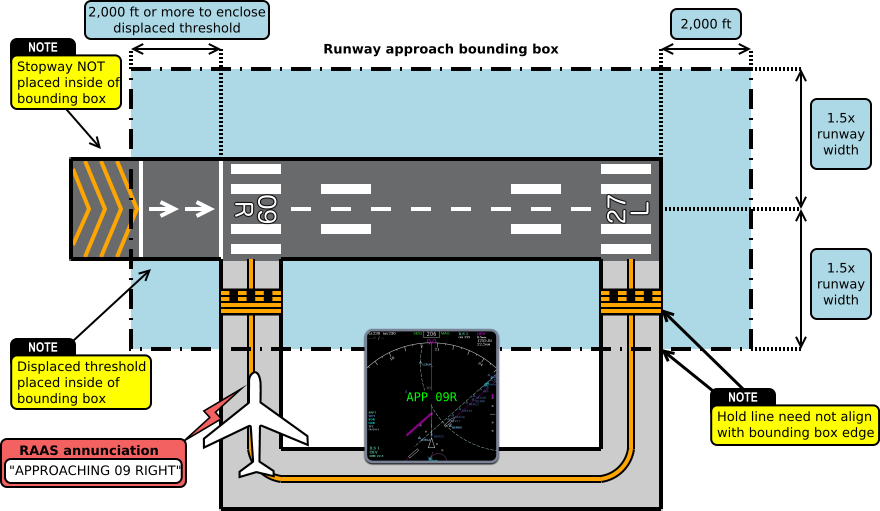
\includegraphics[width=\textwidth]{../src/apch.pdf}
\end{center}
\caption{Approaching a runway on the ground}
\end{figure}

\noindent The aural advisory is accompanied by a routine green visual
advisory on the ND:

\visualadvisory{routine}{APP XX}

\noindent Where `XX' is the runway identifier. The advisory is inhibited
when ground speed exceeds 40 knots to prevent activation on takeoff and
landing through intersecting runways. Please also note that the
annunciation does not guarantee the ability to stop before entering the
runway.

\newpage

\subsection{Lined up on runway for takeoff}
\label{subsec:OnRwyMon}

\begin{wrapfigure}{r}{0.5\textwidth}
\begin{center}
\includegraphics[width=0.5\textwidth]{../src/on_rwy.pdf}
\end{center}
\caption{Lined up on runway for takeoff}
\end{wrapfigure}

This annunciation is made initially on lining up on a runway (aircraft
heading is within 20 degrees of runway heading).  The aural advisory is
accompanied by a routine green visual advisory:

\visualadvisory{routine}{ON XX}

\noindent Where `XX' is the runway identifier. This annunciation may be
supplemented by an annunciation of ``FLAPS, FLAPS'' if the appropriate
takeoff flap configuration has not yet been selected at the time of line
up. The takeoff flaps advisory is inhibited if the GPWS flaps override
mode is active. If the ``FLAPS, FLAPS'' annunciation is to be issued, an
amber non-routine `FLAPS' visual advisory will be issued instead of the
green `ON XX' advisory:

\visualadvisory{nonroutine}{FLAPS}

\subsection{Extended holding on a runway}
\label{subsec:ExtHoldingMon}

If the aircraft holds in position on a runway for an extended period of
time, the on-runway annunciation repeats as a non-routine advisory at
configurable intervals. Holding in position is defined as the aircraft
being aligned with a runway while its ground speed doesn't exceed 4
knots. The aural annunciation is repeated twice per interval (e.g. ``ON
RUNWAY 09 RIGHT, ON RUNWAY 09 RIGHT'') and displays an amber non-routine
`ON XX' visual advisory. The default intervals are defined as follows:

\begin{itemize}

\item Delay until the initial annunciation: 60 seconds

\item Delay until repeat annunciation: 120 seconds

\item Maximum number of annunciations: 3

\end{itemize}

\noindent After the advisory has been repeated for the maximum number of
times, further advisories are inhibited until the aircraft lines up on
another runway. Thus, with the default configuration, the annunciations
occur after holding in position for 1 minute, 3 minutes and 5 minutes.
Refer to section \ref{sec:Configuration} for the interval configuration
parameters
\confopt{on\_rwy\_warn\_initial},
\confopt{on\_rwy\_warn\_repeat} and \confopt{on\_rwy\_warn\_max\_n}.

\newpage
\subsection{Lined up on runway too short for takeoff}
\label{subsec:OnRwyShortMon}

\begin{wrapfigure}{r}{0.5\textwidth}
\vspace{-2em}
\begin{center}
\includegraphics[width=0.5\textwidth]{../src/on_rwy_short.pdf}
\end{center}
\caption{Lined up on runway too short for takeoff}
\vspace{-2em}
\end{wrapfigure}

If the runway length remaining for takeoff is below an operator-defined
minimum for a safe takeoff, the ``ON RUNWAY'' annunciation described in
subsection \ref{subsec:OnRwyMon} is supplemented by a runway distance
remaining readout, rounded down to the nearest 100 feet or meters. The
aural advisory is accompanied by a non-routine amber visual advisory on
the ND:

\visualadvisory{nonroutine}{ON XX YY}

\noindent Where `XX' is the runway identifier and `YY' is the runway
length remaining in hundreds of feet or meters.

\subsection{Short runway takeoff}
\label{subsec:ShortRwyTakeoffMon}

\begin{wrapfigure}{r}{0.5\textwidth}
\vspace{-2em}
\begin{center}
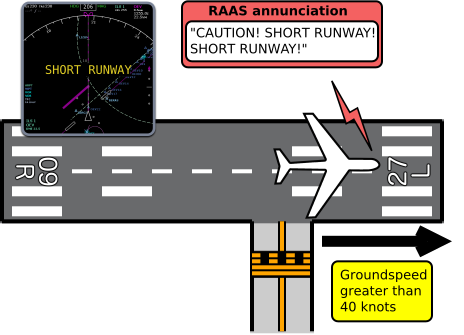
\includegraphics[width=0.5\textwidth]{../src/rwy_short_takeoff.pdf}
\end{center}
\caption{Short runway takeoff}
\vspace{-2em}
\end{wrapfigure}

If takeoff is attempted on a runway with runway length remaining below an
operator defined minimum, once ground speed exceeds 40 knots, a caution
annunciation is generated: ``CAUTION! SHORT RUNWAY! SHORT RUNWAY!'' The
aural advisory is accompanied by a caution amber visual advisory on the
ND:

\visualadvisory{nonroutine}{SHORT RUNWAY}

\subsection{Taxiway takeoff}
\label{subsec:TwyTakeoffMon}

\begin{wrapfigure}{r}{0.5\textwidth}
\vspace{-4em}
\begin{center}
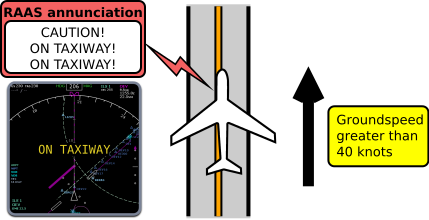
\includegraphics[width=0.5\textwidth]{../src/twy_takeoff.pdf}
\end{center}
\caption{Taxiway takeoff}
\vspace{-4em}
\end{wrapfigure}

This annunciation warns of attempting takeoff on a taxiway, typically
after missing a turn onto the intended departure runway. The conditions
for triggering this annunciation are:

\begin{itemize}

\item the aircraft is NOT on a runway, and

\item ground speed exceeds 40 knots.

\end{itemize}

\noindent The aural advisory is accompanied by a caution amber visual
advisory on the ND:

\visualadvisory{nonroutine}{ON TAXIWAY}

\newpage
\subsection{Late rotation on takeoff}
\label{subsec:LateRotationMon}

\begin{wrapfigure}{r}{0.5\textwidth}
\begin{center}
\includegraphics[width=0.5\textwidth]{../src/takeoff_roll.pdf}
\end{center}
\caption{Late rotation on takeoff}
\end{wrapfigure}

If the aircraft is on a runway and accelerates past 40 knots ground
speed, X-RAAS switches into takeoff mode. Normally most annunciations are
inhibited during this mode, however, if the runway length remaining drops
below an operator-defined value and rotation has not yet been initiated,
X-RAAS will start to issue runway length remaining annunciations to
notify the crew of the rapidly approaching runway end and the need to
initiate rotation as soon as possible. No visual advisories are
generated.

\subsection{Rejected takeoff}
\label{subsec:RejectedTakeoffMon}

In takeoff mode (on runway and ground speed greater than 40 knots),
X-RAAS closely monitors the aircraft's ground speed. If the aircraft
decelerates 5 knots below the maximum ground speed attained during the
takeoff roll, X-RAAS assumes that the takeoff is being rejected. During a
rejected takeoff, if runway length remaining decreases below 9000 feet or
2700 meters, X-RAAS will start to issue runway length remaining
annunciations.  No visual advisories are generated.

\begin{figure}[H]
\begin{center}
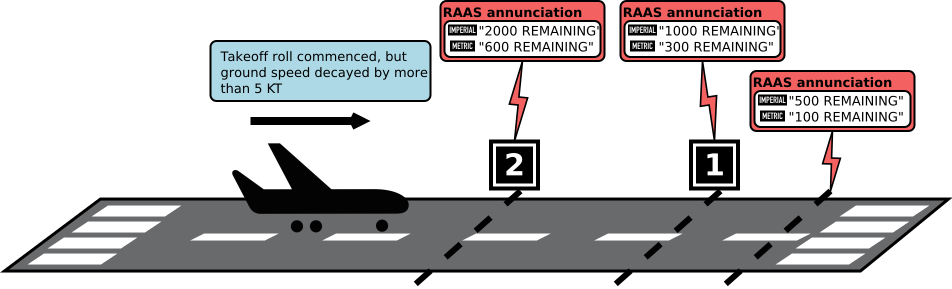
\includegraphics[height=4.5cm]{../src/takeoff_rejected.pdf}
\end{center}
\caption{Rejected takeoff}
\end{figure}

\newpage
\subsection{Altimeter setting climbing through transition altitude}
\label{subsec:AltmQNEMon}

X-RAAS determines the transition altitude based on database information
for the closest airport to the aircraft. If the aircraft climbs through
the transition altitude, X-RAAS monitors the barometric altimeter
subscale setting. If by 30 seconds after transitioning the subscale is
not set to QNE (1013.25 hPa or 29.92 in.Hg), the following advisory is
issued: ``ALTIMETER SETTING''. This is to prevent incorrect altitude
readings in cruise, which increases the possibility of traffic
collisions. The aural advisory is accompanied by a caution amber visual
advisory on the ND:

\visualadvisory{nonroutine}{ALTM SETTING}

\noindent Please note that this advisory might not be available if
transition altitude is not published in the navigation database. Flight
crews must remain fully alert to crossing the transition altitude and
reliance on the altimeter setting RAAS annunciation as part of standard
operations is prohibited.

\begin{figure}[H]
\begin{center}
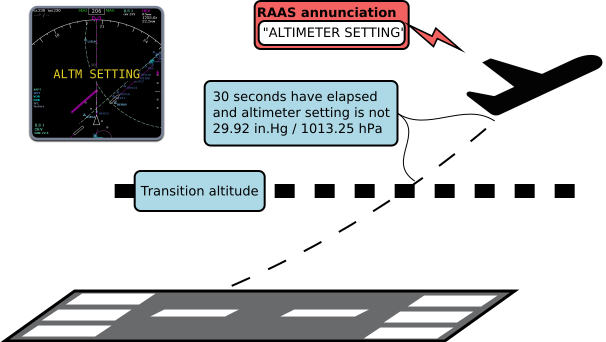
\includegraphics[width=0.8\textwidth]{../src/alt_setting_clb.pdf}
\end{center}
\caption{Altimeter setting climbing through transition altitude}
\end{figure}

\newpage
\subsection{Altimeter setting descending through transition level}
\label{subsec:AltmQNHQFEMon}

This is the reverse advisory to the altimeter setting advisory during
climb. X-RAAS determines the transition level based on the navigational
database entries of the airport closest to the aircraft. If a fixed
transition level is not published, X-RAAS calculates the lowest possible
transition level based on barometric pressure readings, GPS calculated
elevation AMSL and a published transition altitude, such that the
calculated transition level is equal in true elevation AMSL to the
transition altitude. Please note that this fallback mechanism might not
be as accurate as using the ATC-assigned transition level, so reliance on
this annunciation to determine the correct transition level is
prohibited.

Once the aircraft descends through the transition level, X-RAAS monitors
the barometric altimeter reading and GPS-calculated altitude:

\begin{itemize}

\item If the QNH altimeter monitor mode is enabled\footnote{See parameter
\confopt{altm\_qnh\_mon} in section \ref{sec:Configuration}.}, the
GPS-determined elevation AMSL is compared to the barometric altimeter
reading. If the values differ by more than a pre-determined threshold
after more than 30 seconds has elapsed since crossing the transition
level, an “ALTIMETER SETTING” annunciation is generated.

\item If the QFE altimeter monitor mode is enabled\footnote{See parameter
\confopt{altm\_qfe\_mon} in section \ref{sec:Configuration}.}, X-RAAS compares
GPS-determined elevation above the nearest aerodrome with the barometric
altimeter reading to make sure that they are within a pre-determined
threshold.

\end{itemize}

\noindent The default altimetry mode is QNH. The 30 second timeout for
the barometric altimeter setting check can be preempted and initiated
early if the aircraft descends below 1,500 feet above field elevation of
the nearest airport.

The aural advisory is accompanied by a caution amber visual advisory on
the ND:

\visualadvisory{nonroutine}{ALTM SETTING}

\begin{figure}[H]
\begin{center}
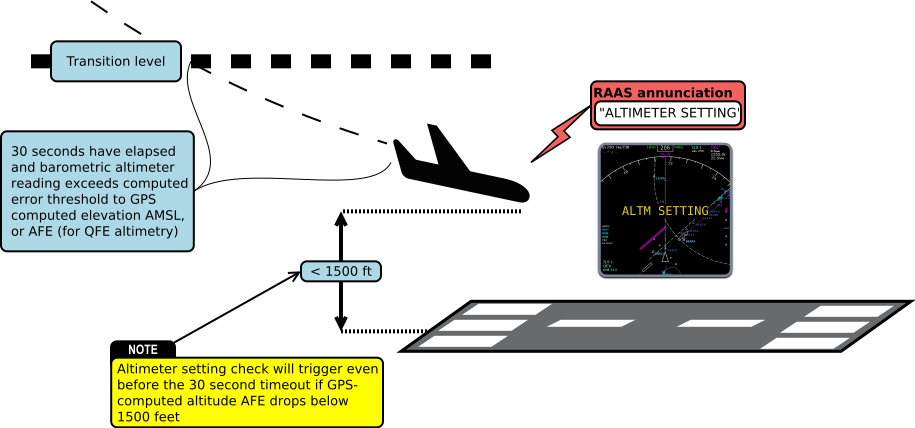
\includegraphics[width=\textwidth]{../src/alt_setting_des.pdf}
\end{center}
\caption{Altimeter setting descending through transition level}
\end{figure}

\subsection{Approaching a runway to land}
\label{subsec:ApchAirMon}

To facilitate proper runway alignment, X-RAAS issues a runway approach
annunciation also when approaching a runway from the air with the
intention to land. The following conditions need to be met for this
annunciation:

\begin{itemize}

\item Within approximately 3 nm of a runway.

\item Track is aligned with the runway and heading is within 20 degrees
of runway heading.

\item In landing configuration.

\item Descending through between 700 feet and 320 feet above runway
threshold elevation\footnote{The annunciation is temporarily inhibited
between 520-480 feet and 420-380 feet above threshold elevation to allow
for GPWS or manual altitude callouts.}.

\end{itemize}

\noindent The aural advisory is accompanied by a routine green visual
advisory on the ND:

\visualadvisory{routine}{APP XX}

\noindent Where `XX' is the runway identifier. If the runway length is
below an operator-defined minimum\footnote{See parameter
\confopt{min\_landing\_dist} in section \ref{sec:Configuration}.}, the
annunciation is supplemented by an additional callout of the length
available for landing, rounded down to the nearest 100 feet or 100
meters. In this case, the following non-routine amber visual advisory
displays on the ND instead:

\visualadvisory{nonroutine}{APP XX YY}

\noindent Where `XX' is the runway identifier and `YY' is the runway
length available in hundreds of feet or meters. If the aircraft remains
on approach, and descends below 400 feet, but is above 320 feet, an
additional annunciation is made: ``CAUTION. SHORT RUNWAY! SHORT RUNWAY!''
This annunciation is accompanied by a caution amber visual advisory:

\visualadvisory{nonroutine}{SHORT RUNWAY}

\begin{figure}[H]
\begin{center}
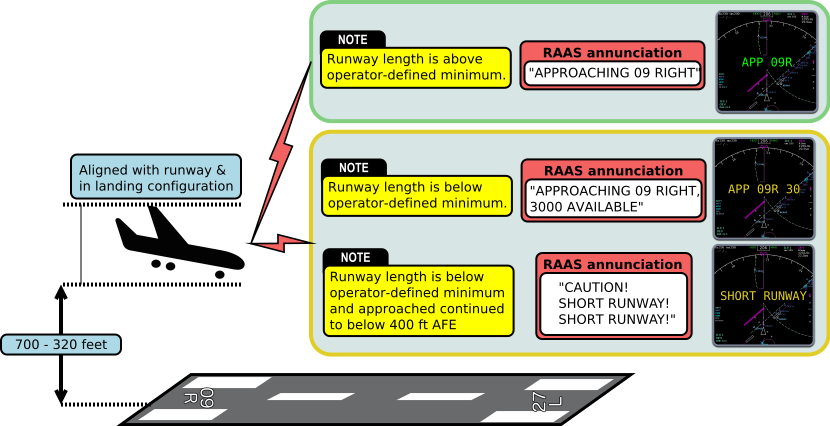
\includegraphics[width=\textwidth]{../src/apch_land.pdf}
\end{center}
\caption{Approaching a runway to land}
\end{figure}

\subsection{Late flap selection during approach to land}
\label{subsec:ApchFlapsMon}

X-RAAS also monitors the flaps configuration\footnote{See parameter
\confopt{min\_landing\_flap} in section \ref{sec:Configuration}.} during an
approach to land and issues flaps advisories in case flaps are not in the
proper setting for landing at certain periods during the approach, based
on height above runway threshold:

\begin{itemize}

\item 950 feet to 600 feet, aural: ``FLAPS (pause) FLAPS'',
visual:\visualadvisory[i]{nonroutine}{FLAPS}

\item 600 feet to 450 feet, aural: ``FLAPS! FLAPS!'',
visual:\visualadvisory[i]{nonroutine}{FLAPS}

\item 450 feet to 300 feet, aural: ``UNSTABLE! UNSTABLE!'',
visual:\visualadvisory[i]{nonroutine}{UNSTABLE}

\end{itemize}

\noindent All visual alerts are generated at the caution level. This
annunciation is inhibited if:

\begin{itemize}

\item the aircraft descends below 300 feet above threshold elevation, or

\item the GPWS flaps override mode (or terrain override mode if the
aircraft isn't equipped with a separate flaps override mode) is active,
or

\item gear is not down, or

\item the rate of climb exceeds 300 feet per minute (go-around
detection).

\end{itemize}

\begin{figure}[H]
\begin{center}
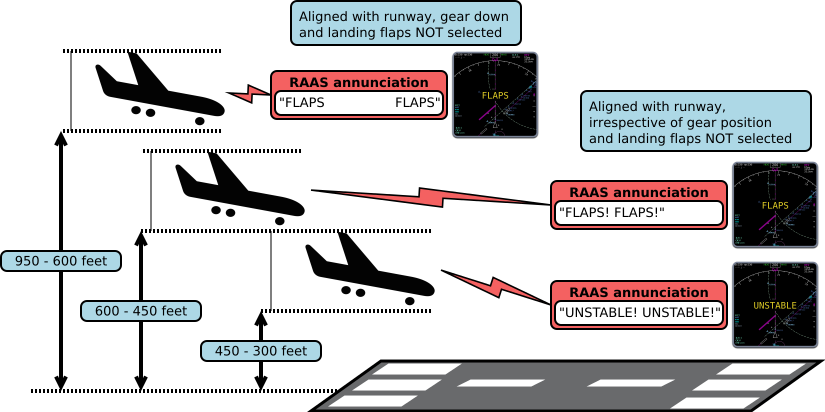
\includegraphics[width=\textwidth]{../src/apch_flaps.pdf}
\end{center}
\caption{Late flap selection during approach to land}
\end{figure}

\subsection{Steep descent late in the approach to land}
\label{subsec:TooHighMon}

To protect against steep descents late in the landing approach and ``dive
bombing it'' at the last moment, X-RAAS calculates the aircraft glide
path angle and compares it with the optimal glide path angle stored in
the database for the runway. If the actual glide path angle exceeds a
limiting angle, X-RAAS issues caution advisories, depending on height
above runway threshold:

\begin{itemize}

\item 950 feet to 600 feet: aural: ``TOO HIGH (pause) TOO HIGH''
visual:\visualadvisory[i]{nonroutine}{TOO HIGH}

\item 600 feet to 450 feet: aural: ``TOO HIGH! TOO HIGH!''
visual:\visualadvisory[i]{nonroutine}{TOO HIGH}

\item 450 feet to 300 feet: aural: ``UNSTABLE! UNSTABLE!''
visual:\visualadvisory[i]{nonroutine}{UNSTABLE}

\end{itemize}

\noindent All visual alerts are generated at the caution level.
Annunciation is inhibited if:

\begin{itemize}

\item the aircraft descends below 300 feet above threshold elevation, or

\item the GPWS terrain override mode is active, or

\item the rate of climb exceeds 300 feet per minute (go-around
detection).

\end{itemize}

\begin{figure}[H]
\begin{center}
\includegraphics[width=\textwidth]{../src/apch_too_hig.pdf}
\end{center}
\caption{Steep descent late in the approach to land}
\end{figure}

\noindent The algorithm for calculating the limiting glide path angle is
based on the aircraft's distance from the runway threshold. The distance
determines a multiplier applied to the optimal angle. For example, if the
multiplier is 2 and the optimal glide path angle is 3\degree, then the
limiting angle is 6\degree\ for that particular point on the approach.
Refer to figure~\ref{fig:GPATable} for details on the actual multiplier
values used.

\begin{figure}[H]
\begin{center}
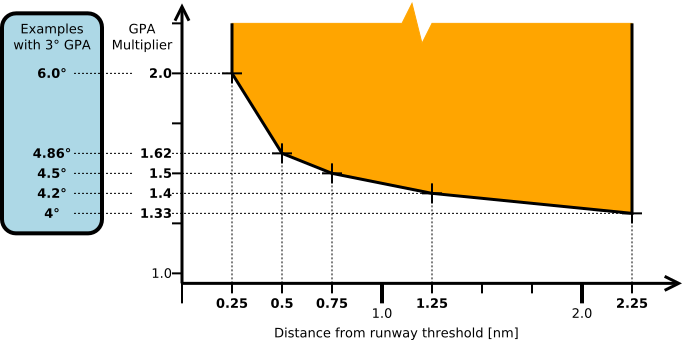
\includegraphics[width=\textwidth]{../src/gpa_mult_table.pdf}
\end{center}
\caption{Glidepath angle multiplier table}
\label{fig:GPATable}
\end{figure}

\subsection{Excessive airspeed on approach}
\label{subsec:TooFastMon}

This check monitors airspeed during an approach and compares it with the
landing speed set in the FMS. If the indicated airspeed becomes excessive
while passing through pre-determined height gates above threshold
elevation, X-RAAS will issue the following annunciations:

\begin{itemize}

\item 950 feet to 600 feet: aural: ``TOO FAST (pause) TOO FAST''
visual:\visualadvisory[i]{nonroutine}{TOO FAST}

\item 600 feet to 450 feet: aural: ``TOO FAST! TOO FAST!''
visual:\visualadvisory[i]{nonroutine}{TOO FAST}

\item 450 feet to 300 feet: aural: ``UNSTABLE! UNSTABLE!''
visual:\visualadvisory[i]{nonroutine}{UNSTABLE}

\end{itemize}

\noindent All visual alerts are generated at the caution level.
Annunciation is inhibited if:

\begin{itemize}

\item the aircraft descends below 300 feet above threshold elevation, or

\item the GPWS terrain or flaps override mode is active, or

\item the rate of climb exceeds 300 feet per minute.

\end{itemize}

\begin{figure}[H]
\begin{center}
\includegraphics[width=\textwidth]{../src/apch_too_fast.pdf}
\end{center}
\caption{Excessive airspeed on approach}
\end{figure}

\noindent The amount of speed margin allowed above the landing speed
depends on the height above the runway threshold and whether the landing
speed includes wind and gust factors (V\textsubscript{APP} –- common on
Airbus) or not (V\textsubscript{REF} –- common on Boeing):

\begin{center}
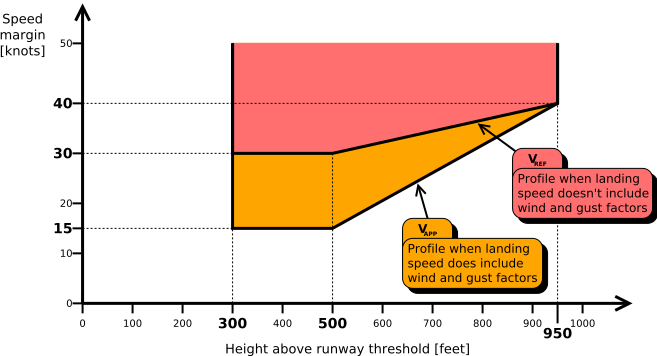
\includegraphics[width=0.8\textwidth]{../src/spd_table.pdf}
\end{center}

\noindent Please note that excessive approach speed monitoring requires
aircraft-specific integration. Refer to section
\ref{sec:Compatibility} for a list of aircraft which support
this feature.

\subsection{Attempting to land on a parallel taxiway}
\label{subsec:TwyLandingMon}

Many airports feature runways with close parallel taxiways. Under certain
conditions, these can look very similar to each other during final
approach and lead to confusion as to which is the runway and which is a
taxiway. This increases the risk of an aircraft attempting to land on a
taxiway.

To help in preventing this hazard, X-RAAS closely monitors an aircraft's
position during the final stages of approach. If X-RAAS detects all of
the following conditions, it will issue a caution advisory:

\begin{itemize}

\item Radio altitude is less than 250 feet, but more than 100 feet.

\item The aircraft is in landing configuration (gear is down and flaps in
the landing position).

\item The aircraft is NOT in the runway approach area \emph{or} it is NOT
aligned with the runway (aircraft heading not within 20 degrees of runway
heading).

\end{itemize}

\noindent The advisory is inhibited if the aircraft descends below 100
feet radio altitude\footnote{If the parallel taxiway is very close to the
runway, X-RAAS may not be able to detect a taxiway landing attempt. This
is due to the minimum radio altitude constraint and the runway approach
area shape. There is a minimum lateral deviation value of the aircraft's
longitudinal center axis from the edge of the runway surface. If the
actual lateral deviation is less than this minimum value, this advisory
is inhibited. For runways with a 3\degree glidepath, a threshold clearing
height of 50 feet and roughly flat terrain in the runway approach area,
the minimum lateral deviation is approximately 56 feet or 17 meters. The
shallower the glidepath or the higher the terrain in the approach area,
the wider the minimum lateral deviation below which this advisory will be
inhibited.}, or if the GPWS terrain override mode is active. The aural
advisory is accompanied by a caution visual advisory:

\visualadvisory{nonroutine}{TAXIWAY}

\begin{figure}[H]
\begin{center}
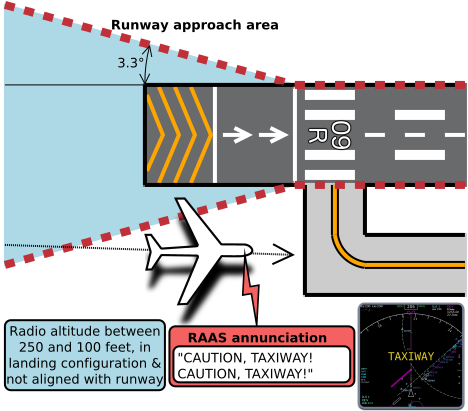
\includegraphics[width=0.6\textwidth]{../src/off_rwy_landing.pdf}
\end{center}
\caption{Attempting to land on a parallel taxiway}
\end{figure}

\subsection{Long landing/Deep landing}
\label{subsec:LongLandingMon}

This annunciation protects against excessive floating on landing or an
incorrectly executed too high or too fast approach, resulting in touch
down very far down the runway and potentially insufficient runway length
available for rollout. For this annunciation to trigger, all of the
following conditions must be met:

\begin{itemize}

\item The aircraft is above the runway.

\item Radio altitude indicates less than 100 feet, but more than 5 feet.

\item Aircraft is past \myfrac{1}{4} of the runway length or 2,000
feet from the approach end (whichever is shorter), or remaining runway
length is less than an operator-defined minimum.

\end{itemize}

\begin{figure}[H]
\begin{center}
\includegraphics[width=\textwidth]{../src/long_land.pdf}
\end{center}
\caption{Long landing}
\end{figure}

\noindent X-RAAS will initially annunciate ``LONG LANDING!'' twice and
the remaining runway length if it is less than 9,000 feet (2,700 meters)
or an operator-defined maximum\footnote{See parameter
\confopt{stop\_dist\_cutoff} in section \ref{sec:Configuration}.}.
Afterwards, X-RAAS will continue to annunciate runway length remaining
every 1,000 feet (300 meters), unless the aircraft lands and decelerates
below 40 knots ground speed, or performs a go-around (refer to section
\ref{subsec:GoAround} for conditions monitored during a go-around). The
aural advisory is accompanied by a caution amber visual advisory on the
ND:

\visualadvisory{nonroutine}{LONG LANDING}

\subsection{Landing rollout runway length remaining}
\label{subsec:LandRolloutMon}

During landing rollout, X-RAAS closely monitors aircraft position, ground
speed and deceleration. X-RAAS will start issuing runway distance
remaining annunciations in 1,000 foot or 300 meter increments if all of
the following conditions are met:

\begin{itemize}

\item the remaining runway length is less than 5,000 feet or 1,500 meters
(configurable as an operator-defined value\footnote{See parameter
\confopt{stop\_dist\_cutoff} in section \ref{sec:Configuration}.}),

\item the ground speed is above 40 knots,

\item the current rate of deceleration is insufficient to come to a
complete stop prior to the end of the runway.

\end{itemize}

\noindent Thus the annunciation of runway length remaining during a
normal landing indicates that additional braking might be required to
bring the aircraft to a safe stop. The runway distance remaining
annunciations are based on the position the aircraft's nosewheel will
attain in approximately 1 second with an added approximate 200 foot or 60
meter buffer. Therefore a ``3000 (feet) remaining'' annunciation can be
sounded between 3,000 to 3,200 feet remaining. The last 1,000 feet or 300
meters of runway length remaining feature two additional annunciations:

\begin{itemize}

\item The last 500 feet or 100 meters. Inhibited if ground speed is below
40 knots.

\item The last 100 feet or 30 meters. This annunciation is sounded
irrespective of ground speed as long as the aircraft remains aligned with
the runway to warn the pilot of the need to perform an immediate stop or
turn to avoid running off the end of the runway.

\end{itemize}

\begin{figure}[H]
\begin{center}
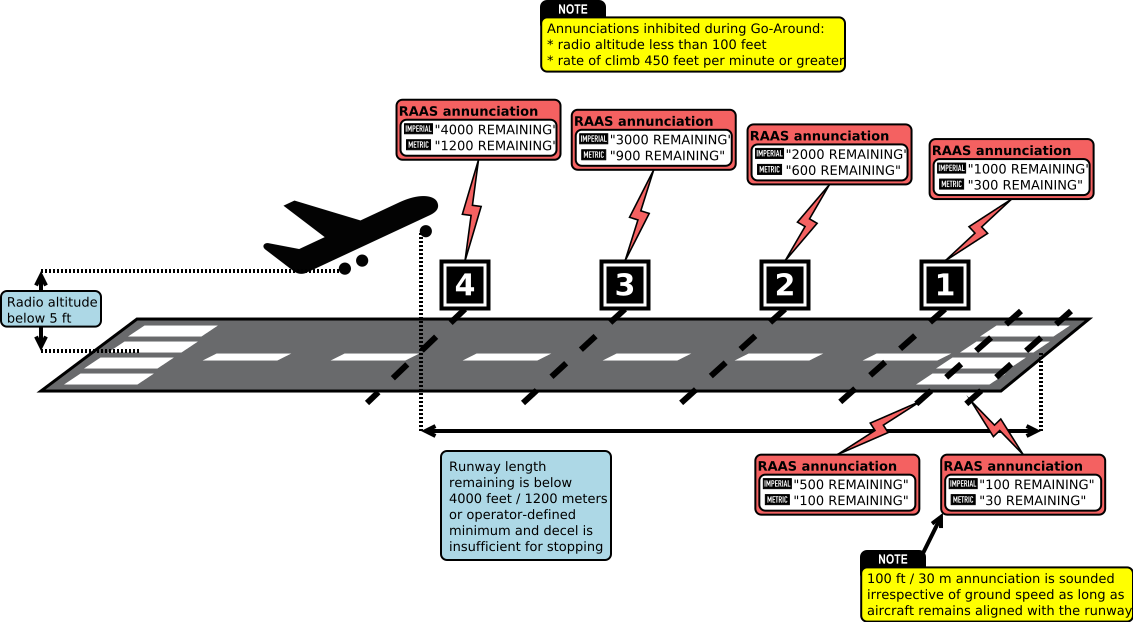
\includegraphics[width=\textwidth]{../src/land_rollout.pdf}
\end{center}
\caption{Landing rollout runway length remaining}
\end{figure}

\noindent The runway length remaining is calculated based on the position
of the threshold of the opposite runway. If the opposite runway features
a displaced threshold, this displacement length is counted towards the
runway length remaining, i.e. the displaced threshold portion of a runway
is considered to be suitable for landing rollout. If the opposite runway
features a stopway (a ``blastpad''), this is NOT counted towards the
runway length remaining\footnote{Stopways are normally designed for
emergency use only.}.  No visual advisories are generated.

\begin{center}
\begin{tabular}[c]{|l|l|l|}
\hline

\rowcolor{tablehdrcolor}

\textbf{Distance [feet]} & \textbf{Distance [meters]} &
\textbf{Maximum ground speed [knots]} \\

\hline

9,000 & 2,700 & 250 \\

\hline

8,000 & 2,400 & 250 \\

\hline

\multicolumn{3}{|c|}{\ldots} \\

\hline

1,000 & 300 & 250 \\

\hline

500 & 100 & 125 \\

\hline

100 & 30 & 60 \\

\hline

\end{tabular}
\end{center}

\subsection{Go-around}
\label{subsec:GoAround}

During go-around, runway length remaining annunciations are inhibited as
soon as the aircraft climbs through 5 feet radio altitude and the
following two conditions are met:

\begin{itemize}

\item radio altitude is below 100 feet

\item rate of climb is 300 feet per minute or greater

\end{itemize}

\noindent If the rate of climb decays to below 300 feet per minute,
runway length remaining annunciations are continued. If the aircraft
climbs through 100 feet radio altitude, runway length remaining
annunciations are not performed even if the aircraft resumes level
flight.

\subsection{Runway exit via high-speed exit taxiways}
\label{subsec:HighSpeedExit}

To support efficient high-traffic-density operations, landing traffic
needs to be able to exit the runway environment after landing in an
expeditious manner. To this end, many airports feature ``high-speed
exit'' taxiways. These taxiways, rather than connecting to the runway at
right angles, connect at relatively shallow angles, allowing landing
traffic to maintain higher speed when turning off the runway. To support
high-speed rollouts onto these kinds of taxiways, X-RAAS monitors
groundspeed and aircraft position relative to the runway after landing.
If the aircraft exceeds a limiting ground speed, this annunciation will
be generated: ``CAUTION! ON TAXIWAY! ON TAXIWAY!'' and
\visualadvisory[i]{nonroutine}{ON TAXIWAY} on the ND.

\begin{itemize}

\item As long as the aircraft remains on a runway, no limiting ground
speed is imposed.

\item If the aircraft leaves the runway, but remains within the runway
approach bounding box (as described in section \ref{subsec:ApchGndMon}),
the limiting ground speed is 60 knots.

\item If the aircraft leaves both the runway and the runway approach
bounding box, the limiting ground speed is 40 knots.

\end{itemize}

\begin{figure}[H]
\begin{center}
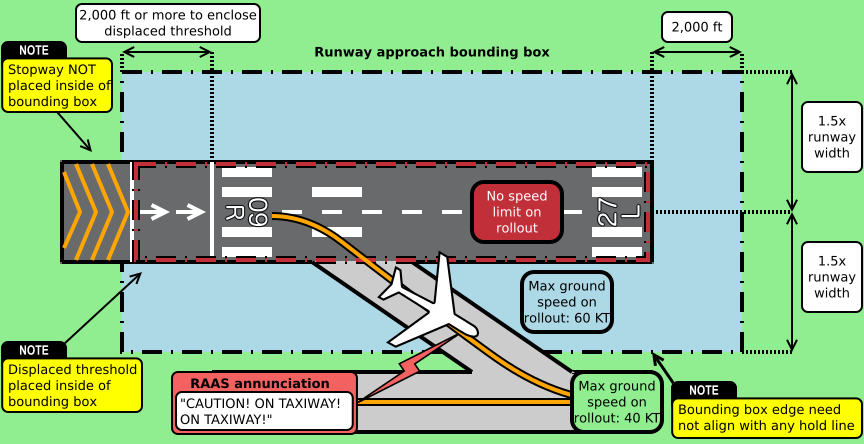
\includegraphics[width=\textwidth]{../src/taxi_offrwy.pdf}
\end{center}
\caption{Runway exit via high-speed exit taxiways}
\end{figure}

\section{Configuration}
\label{sec:Configuration}

Just like the real system, X-RAAS can be extensively customized to suit
the particular operational requirements of an aircraft or airline. For
this purpose, X-RAAS contains both a graphical and textual configuration
interface. Both interfaces have equivalent capability. The graphical
configuration system simply generates a text configuration that is then
stored on disk and read by X-RAAS during startup.

\subsection{Graphical configuration}
\label{subsec:GUIConfiguration}

To invoke the graphical configuration interface, choose
``Plugins''$\rightarrow$``X-RAAS''$\rightarrow$``X-RAAS configuration\ldots''
from the simulator's main menu. This will bring up the main
configuration window shown in figure \ref{GUIConfigurationWindow}.

\begin{figure}[H]
\vspace{.5em}
\begin{center}
\includegraphics[width=\textwidth]{../src/config_window_annotated.png}
\end{center}
\caption{Graphical configuration}
\label{GUIConfigurationWindow}
\end{figure}

\noindent When open, the window will reflect the state of the current
configuration of X-RAAS. You can make changes to the configuration and
save it, or reset it to a default state. The following table explains
what every control in the configuration window does:

\newcommand{\guiconfbtn}[1]{#1\label{gui_conf_btn_label_#1}}

{\footnotesize
\begin{center}
\tablefirsthead{%
\hline
\rowcolor{tablehdrcolor}
\multicolumn{1}{|c}{\textbf{\#}} &
\multicolumn{1}{|c}{\textbf{Description}} &
\multicolumn{1}{|c}{\textbf{Default}} &
\multicolumn{1}{|p{4cm}|}{\textbf{Equivalent text config param}} \\
\hline}
\tablehead{%
\hline
\rowcolor{tablecontcolor}
\multicolumn{4}{|l|}{\sl continued from previous page}\\ \hline
\rowcolor{tablehdrcolor}
\multicolumn{1}{|c}{\textbf{\#}} &
\multicolumn{1}{|c}{\textbf{Description}} &
\multicolumn{1}{|c}{\textbf{Default}} &
\multicolumn{1}{|p{4.6cm}|}{\textbf{Equivalent text config param}} \\ }
\tabletail{%
\hline
\rowcolor{tablecontcolor}
\multicolumn{4}{|r|}{\sl continued on next page}\\
\hline}
\tablelasttail{\hline}
\begin{supertabular}{|c|p{8cm}|c|l|}

\guiconfbtn{1} &
The master ON/OFF switch.\newline
\textbf{ON:} X-RAAS starts up if the current aircraft is compatible.\newline
\textbf{OFF:} X-RAAS startup is completely inhibited. &
\textbf{ON} &
\confopt{enabled} \\

\hline

\guiconfbtn{2} &
Switches the unit of measure for distances used.\newline
\textbf{ON:} use feet as the unit of measure in annunciations.\newline
\textbf{OFF:} use meters as the unit of measure in annunciations.\newline
This setting doesn't affect the units used in the configuration
interface. The configuration interface always requires lengths and
distances to be specified in meters. & \textbf{ON} &
\confopt{use\_imperial} \\

\hline

\guiconfbtn{3} &
X-RAAS has the option of pronouncing single-digit runways with or without
prepending a leading '0'. Prepending '0' is ICAO-standard nomenclature,
whereas not prepending '0' is used in FAA-governed territories.\newline
\textbf{ON:} pronounce single-digit runway numbers without a leading `0'
(e.g. `1L').\newline
\textbf{OFF:} pronounce single-digit runway numbers with a leading `0'
(e.g. `01L'). & \textbf{OFF} & \confopt{us\_runway\_numbers} \\

\hline

\guiconfbtn{4} &
Sets the aural annunciation voice gender.\newline
\textbf{ON:} the voice of aural annunciations is female.\newline
\textbf{OFF:} the voice of aural annunciations is male. &
\textbf{ON} & \confopt{voice\_female} \\

\hline

\guiconfbtn{5} &
During runway distance remaining or available annunciations, selects
whether the units of measure used in the annunciation are appended to the
initial annunciation (subsequent annunciations omit the units).\newline
\textbf{ON:} append the units of measure used to initial distance
annunciations.\newline
\textbf{OFF:} don't append the units of measure used to distance
annunciations. & \textbf{ON} & \confopt{speak\_units} \\

\hline

\guiconfbtn{6} &
If a late touchdown on landing is detected, this setting controls what
nomenclature is used to annunciate this fact:\newline
\textbf{ON:} annunciate late touchdown as `DEEP LANDING'.\newline
\textbf{OFF:} annunciate late touchdown as `LONG LANDING'.\newline
This setting does not control whether the long landing monitor is
enabled. Refer to section \ref{subsec:LongLandingMon} for more information. &
\textbf{OFF} & \confopt{say\_deep\_landing} \\

\hline

\guiconfbtn{7} &

Controls whether X-RAAS startup is allowed if the current aircraft is
detected to be a helicopter.\newline
\textbf{ON:} permit startup if the current aircraft is a helicopter.\newline
\textbf{OFF:} inhibit startup if the current aircraft is a helicopter.\newline
This setting doesn't affect other compatibility checks, such as the
minimum number of engines allowed or the minimum MTOW limit. Refer to
section \ref{subsec:AircraftTypes} for more information.\newline
NOTE: this option is omitted when X-RAAS is distributed as part of an
aircraft package. & \textbf{OFF} &
\confopt{allow\_helos} \\

\hline

\guiconfbtn{8} &
On startup, X-RAAS displays a message at the bottom of the screen for 4
seconds to indicate that it is operating correctly and what units of
measure are used for distance callouts, e.g:
\begin{itemize}
\item ``Runway Awareness OK, Feet.''
\item ``Runway Awareness OK, Meters.''
\end{itemize}
\textbf{ON:} display of the startup message is enabled.\newline
\textbf{OFF:} display of the startup message is inhibited.\newline
This setting doesn't control startup of X-RAAS itself.\newline
NOTE: this option is omitted when X-RAAS is distributed as part of an
aircraft package. & \textbf{ON} &
\confopt{startup\_notify} \\

\hline

\guiconfbtn{9} &
When the currently loaded aircraft doesn't meet the minimum requirements
for X-RAAS to activate, X-RAAS displays a short message at the bottom of
the screen to point out that it is auto-inhibited. This option controls
whether this auto-inhibition message isdisplayed.\newline
\textbf{ON:} the display of the auto-inhibition message is enabled.\newline
\textbf{OFF:} the display of the auto-inhibition message is disabled.\newline
NOTE: this option is omitted when X-RAAS is distributed as part of an
aircraft package. &
\textbf{ON} & \confopt{auto\_disable\_notify} \\

\hline

\guiconfbtn{10} &
\textbf{ON:} while the simulator view is external, audible playback and
display of visual overlay annunciations is inhibited.\newline
\textbf{OFF:} while the simulator view is external, audible playback and
display of visual overlay annunciations is permitted. & \textbf{ON} &
\confopt{disable\_ext\_view} \\

\hline

\guiconfbtn{11} &
Controls whether the issuing of visual annunciations is enabled,
irrespective of whether on the fallback screen overlay or on the
aircraft's ND.\newline
\textbf{ON:} permit issuing visual alerts on the ND or the screen
overlay.\newline
\textbf{OFF:} inhibit issuing visual alerts on the ND and the screen
overlay.\newline
Refer to section \ref{subsec:VisualAnnunciations} for more information. &
\textbf{ON} & \confopt{nd\_alerts\_enabled} \\

\hline

\guiconfbtn{12} &
Controls whether visual annunciations are allowed to be displayed using
the fallback screen overlay.\newline
\textbf{ON:} permit display of visual alerts using the screen
overlay.\newline
\textbf{OFF:} inhibit display of visual alerts using the on-screen
overlay.\newline
This doesn't inhibit the issuing of visual alerts, only their display on
the overlay. If the aircraft model provides display of visual alerts in
the virtual cockpit, those will be displayed even if this setting is set
to OFF. Refer to section \ref{subsec:VisualAnnunciations} for more
information. & \textbf{ON} & \confopt{nd\_alert\_overlay\_enabled} \\

\hline

\guiconfbtn{13} &
On aircraft which provide visual alert integration into the visual
cockpit, X-RAAS will attempt to avoid showing the fallback screen overlay
so as not to disturb the pilot by duplicate messages out of the virtual
instrument frame. This setting allows you to override this behavior and
force the display of the screen overlay.\newline
\textbf{ON:} permit display of visual alerts using the fallback on-screen
overlay.\newline
\textbf{OFF:} inhibit display of visual alerts using the on-screen
overlay.\newline
Refer to section \ref{subsec:VisualAnnunciations} for more information. &
\textbf{OFF} & \confopt{nd\_alert\_overlay\_force} \\

\hline

\guiconfbtn{14} &
Some aircraft models do not properly set the required datarefs for X-RAAS
to detect electrical power being applied to the aircraft's avionics
systems, resulting in X-RAAS being inoperable.\newline
\textbf{ON:} permit startup even if insufficient power is being applied to
the aircraft's electrical buses.\newline
\textbf{OFF:} inhibit startup unless sufficient power is being applied to
the aircraft's electrical buses. & \textbf{OFF} &
\confopt{override\_electrical} \\

\hline

\guiconfbtn{15} &
During replays, aircraft position can behave in strange and
non-predictable ways, which can cause X-RAAS to give spurious
annunciations.\newline
\textbf{ON:} permit X-RAAS operation even if the simulator is currently in
replay mode.\newline
\textbf{OFF:} inhibit X-RAAS operation if the simulator is currently in
replay mode. & \textbf{OFF} & \confopt{override\_replay} \\

\hline

\guiconfbtn{16} &
In case you encounter compatibility issues with audio playback from
X-RAAS and any other remedy is unavailable, you can force X-RAAS to play
aural annunciations using the host operating system's text-to-speech
function.\newline
\textbf{ON:} use the host operating system's text-to-speech function.\newline
\textbf{OFF:} use X-RAAS's own audio playback.\newline
NOTE: this feature is not available on Linux. & \textbf{OFF} &
\confopt{use\_tts} \\

\hline

\guiconfbtn{17} &
When generating audio, X-RAAS can either use a dedicated OpenAL audio
context, or a context shared with the rest of X-Plane. Certain audio
drivers on Windows are known not to properly support multiple OpenAL
contexts. If you encounter audio playback issues in that case, try to
switch X-RAAS to use a shared audio context.\newline
\textbf{ON:} X-RAAS should use an OpenAL audio driver context shared with
the rest of X-Plane.\newline
\textbf{OFF:} X-RAAS should use its own dedicated OpenAL audio driver
context.\newline
NOTE: operating using a shared context can result in compatibility issues
with certain 3rd party plugins and aircraft. & \textbf{OFF} &
\confopt{openal\_shared} \\

\hline

\guiconfbtn{18} &
\textbf{ON:} the approaching runway on ground monitor is enabled.\newline
\textbf{OFF:} the approaching runway on-ground monitor is disabled.\newline
Refer to section \ref{subsec:ApchGndMon} for more information. &
\textbf{ON} & \confopt{apch\_rwy\_on\_gnd\_mon} \\

\hline

\guiconfbtn{19} &
\textbf{ON:} the approaching runway in air monitor is enabled.\newline
\textbf{OFF:} the approaching runway in air monitor is disabled.\newline
Refer to section \ref{subsec:ApchAirMon} for more information. &
\textbf{ON} & \confopt{apch\_rwy\_in\_air\_mon} \\

\hline

\guiconfbtn{20} &
\textbf{ON:} the approaching short runway in air monitor is enabled.\newline
\textbf{OFF:} the approaching short runway in air monitor is disabled.\newline
Refer to section \ref{subsec:ApchAirMon} for more information. & \textbf{ON} &
\confopt{apch\_rwy\_in\_air\_short\_mon} \\

\hline

\guiconfbtn{21} &
\textbf{ON:} the on-runway lineup monitor is enabled.\newline
\textbf{OFF:} the on-runway lineup monitor is disabled.\newline
Refer to section \ref{subsec:OnRwyMon} for more information. &
\textbf{ON} & \confopt{on\_rwy\_lineup\_mon} \\

\hline

\guiconfbtn{22} &
\textbf{ON:} the on-runway (short runway) lineup monitor is enabled.\newline
\textbf{OFF:} the on-runway (short runway) lineup monitor is disabled.\newline
Refer to section \ref{subsec:OnRwyShortMon} for more information. &
\textbf{ON} & \confopt{on\_rwy\_lineup\_short\_mon} \\

\hline

\guiconfbtn{23} &
\textbf{ON:} the on-runway lineup late flap selection monitor is
enabled.\newline
\textbf{OFF:} the on-runway lineup late flap selection monitor is
disabled.\newline Refer to section \ref{subsec:OnRwyMon} for more
information. & \textbf{ON} & \confopt{on\_rwy\_lineup\_flaps\_mon} \\

\hline

\guiconfbtn{24} &
\textbf{ON:} the short runway takeoff monitor is enabled.\newline
\textbf{OFF:} the short runway takeoff monitor is disabled.\newline
Refer to section \ref{subsec:ShortRwyTakeoffMon} for more information. &
\textbf{ON} & \confopt{on\_rwy\_tkoff\_short\_mon} \\

\hline

\guiconfbtn{25} &
\textbf{ON:} the on-runway extended holding monitor is enabled.\newline
\textbf{OFF:} the on-runway extended holding monitor is disabled.\newline
Refer to section \ref{subsec:ExtHoldingMon} for more information. &
\textbf{ON} & \confopt{on\_rwy\_hold\_mon} \\

\hline

\guiconfbtn{26} &
\textbf{ON:} the taxiway takeoff monitor is enabled.\newline
\textbf{OFF:} the taxiway takeoff monitor is disabled.\newline
Refer to section \ref{subsec:TwyTakeoffMon} for more information. &
\textbf{ON} & \confopt{twy\_tkoff\_mon} \\

\hline

\guiconfbtn{27} &
\textbf{ON:} distance remaining callouts on landing are enabled.\newline
\textbf{OFF:} distance remaining callouts on landing are disabled.\newline
Refer to section \ref{subsec:LandRolloutMon} for more information. &
\textbf{ON} & \confopt{dist\_rmng\_land\_mon} \\

\hline

\guiconfbtn{28} &
\textbf{ON:} distance remaining callouts on rejected takeoff are
enabled.\newline
\textbf{OFF:} distance remaining callouts on rejected takeoff are
disabled.\newline
Refer to section \ref{subsec:RejectedTakeoffMon} for more information. &
\textbf{ON} & \confopt{dist\_rmng\_rto\_mon} \\

\hline

\guiconfbtn{29} &
\textbf{ON:} the taxiway landing monitor is enabled.\newline
\textbf{OFF:} the taxiway landing monitor is disabled.\newline
Refer to section \ref{subsec:TwyLandingMon} for more information. &
\textbf{ON} & \confopt{twy\_land\_mon} \\

\hline

\guiconfbtn{30} &
\textbf{ON:} the runway ending distance remaining callout is enabled.\newline
\textbf{OFF:} the runway ending distance remaining callout is disabled. &
\textbf{ON} & \confopt{rwy\_end\_mon} \\

\hline

\guiconfbtn{31} &
\textbf{ON:} the `TOO HIGH' approach monitor upper gate (950-600 ft AFE)
is enabled.\newline
\textbf{OFF:} the `TOO HIGH' approach monitor upper gate is disabled.\newline
Refer to section \ref{subsec:TooHighMon} for more information. &
\textbf{ON} & \confopt{apch\_too\_high\_upper\_mon} \\

\hline

\guiconfbtn{32} &
\textbf{ON:} the `TOO HIGH' approach monitor lower gate (600-450 ft AFE)
is enabled.\newline
\textbf{OFF:} the `TOO HIGH' approach monitor lower gate is disabled.\newline
Refer to section \ref{subsec:TooHighMon} for more information. &
\textbf{ON} & \confopt{apch\_too\_high\_lower\_mon} \\

\hline

\guiconfbtn{33} &
\textbf{ON:} the `TOO FAST' approach monitor upper gate (950-600 ft AFE)
is enabled.\newline
\textbf{OFF:} the `TOO FAST' approach monitor upper gate is disabled.\newline
Refer to section \ref{subsec:TooFastMon} for more information. &
\textbf{ON} & \confopt{apch\_too\_fast\_upper\_mon} \\

\hline

\guiconfbtn{34} &
\textbf{ON:} the `TOO FAST' approach monitor lower gate (600-450 ft AFE)
is enabled.\newline
\textbf{OFF:} the `TOO FAST' approach monitor lower gate is disabled.\newline
Refer to section \ref{subsec:TooFastMon} for more information. &
\textbf{ON} & \confopt{apch\_too\_fast\_lower\_mon} \\

\hline

\guiconfbtn{35} &
\textbf{ON:} the late flap selection approach monitor upper gate
(950-600 ft AFE) is enabled.\newline
\textbf{OFF:} the late flap selection approach monitor upper gate is
disabled.\newline
Refer to section \ref{subsec:ApchFlapsMon} for more information. &
\textbf{ON} & \confopt{apch\_flaps\_upper\_mon} \\

\hline

\guiconfbtn{36} &
\textbf{ON:} the late flap selection approach monitor lower gate
(600-450 ft AFE) is enabled.\newline
\textbf{OFF:} the late flap selection approach monitor lower gate is
disabled.\newline
Refer to section \ref{subsec:ApchFlapsMon} for more information. &
\textbf{ON} & \confopt{apch\_flaps\_lower\_mon} \\

\hline

\guiconfbtn{37} &
The conditions checked depend on the lower gate setting of the respective
approach monitor.\newline
\textbf{ON:} the unstable approach monitor is enabled.\newline
\textbf{OFF:} the unstable approach monitor is disabled.\newline
Refer to sections \ref{subsec:TooHighMon}, \ref{subsec:TooFastMon} and
\ref{subsec:ApchFlapsMon} for more information. & \textbf{ON} &
\confopt{apch\_unstable\_mon} \\

\hline

\guiconfbtn{38} &
\textbf{ON:} the QNE altimeter setting monitor mode is enabled.\newline
\textbf{OFF:} the QNE altimeter setting monitor mode is disabled.\newline
Refer to section \ref{subsec:AltmQNEMon} for more information. &
\textbf{ON} & \confopt{altm\_qne\_mon} \\

\hline

\guiconfbtn{39} &
\textbf{ON:} the QNH altimeter setting monitor mode is enabled.\newline
\textbf{OFF:} the QNH altimeter setting monitor mode is disabled.\newline
Refer to section \ref{subsec:AltmQNHQFEMon} for more information. &
\textbf{ON} & \confopt{altm\_qnh\_mon} \\

\hline

\guiconfbtn{40} &
\textbf{ON:} the QFE altimeter setting monitor mode is enabled.\newline
\textbf{OFF:} the QFE altimeter setting monitor mode is disabled.\newline
Refer to section \ref{subsec:AltmQNHQFEMon} for more information. &
\textbf{OFF} & \confopt{altm\_qfe\_mon} \\

\hline

\guiconfbtn{41} &
\textbf{ON:} the long landing monitor is enabled.\newline
\textbf{OFF:} the long landing monitor is disabled.\newline
Refer to section \ref{subsec:LongLandingMon} for more information. &
\textbf{ON} & \confopt{long\_land\_mon} \\

\hline

\guiconfbtn{42} &
\textbf{ON:} the late rotation on takeoff monitor is enabled.\newline
\textbf{OFF:} the late rotation on takeoff monitor is disabled.\newline
Refer to section \ref{subsec:LateRotationMon} for more information. &
\textbf{ON} & \confopt{late\_rotation\_mon} \\

\hline

\guiconfbtn{43} & The relative audio volume for aural annunciations. &
\textbf{100} & \confopt{voice\_volume} \\

\hline

\guiconfbtn{44} &
Minimum number of engines the aircraft must have for it to be considered
an ``airliner'' and permit X-RAAS startup.\newline
NOTE: this option is omitted when X-RAAS is distributed as part of an
aircraft package. &
\textbf{2} &
\confopt{min\_engines} \\

\hline

\guiconfbtn{45} &
Lowest value of the aircraft's Maximum TakeOff Weight (MTOW) for it to be
considered an ``airliner'' and permit X-RAAS startup.\newline
NOTE: this option is omitted when X-RAAS is distributed as part of an
aircraft package. &
\textbf{5700} & \confopt{min\_takeoff\_dist} \\

\hline

\guiconfbtn{46} &
The minimum runway length remaining that is considered to be safe for
conducting a takeoff. If the runway length remaining is less than this
value, caution annunciations will be issued.\newline
Refer to section \ref{subsec:ExtHoldingMon} for more information. &
\textbf{1000} & \confopt{min\_landing\_dist} \\

\hline

\guiconfbtn{47} &
The minimum runway length remaining that is considered to be safe for
conducting a landing. If the runway length remaining is less than this
value, caution annunciations will be issued.\newline
Refer to section \ref{subsec:ApchAirMon} for more information. &
\textbf{800} & \confopt{min\_landing\_dist} \\

\hline

\guiconfbtn{48} &
The minimum runway length remaining by which if the aircraft hasn't
initiated rotation, X-RAAS will start issuing runway length remaining
annunciations to warn of rapidly approaching the runway end.\newline
Refer to section \ref{subsec:LateRotationMon} for more information. &
\textbf{400} & \confopt{min\_rotation\_dist} \\

\hline

\guiconfbtn{49} &
The minimum pitch angle relative to the runway slope above which X-RAAS
considers the aircraft to have initiated rotation for takeoff.\newline
Refer to section \ref{subsec:LateRotationMon} for more information. &
\textbf{3} & \confopt{min\_rotation\_angle} \\

\hline

\guiconfbtn{50} &
On landing, do not initiate runway length remaining annunciations as long
as the runway length remaining is above this value.\newline
Refer to section \ref{subsec:LandRolloutMon} for more information. &
\textbf{1600} & \confopt{dist\_dist\_cutoff} \\

\hline

\guiconfbtn{51} &
Issue the first ``ON RUNWAY'' annunciation for extended holding on the
runway after this number of seconds have elapsed.\newline
Refer to section \ref{subsec:ExtHoldingMon} for more information. &
\textbf{60} & \confopt{on\_rwy\_warn\_initial} \\

\hline

\guiconfbtn{52} &
Issue subsequent ``ON RUNWAY'' annunciations for extended holding on the
runway after this number of seconds have elapsed.\newline
Refer to section \ref{subsec:ExtHoldingMon} for more information. &
\textbf{120} & \confopt{on\_rwy\_warn\_repeat} \\

\hline

\guiconfbtn{53} &
Maximum number of ``ON RUNWAY'' annunciations issued for extended holding
on the runway.
Refer to section \ref{subsec:ExtHoldingMon} for more information. &
\textbf{3} & \confopt{on\_rwy\_warn\_max\_n} \\

\hline

\guiconfbtn{54} &
Maximum glidepath angle multiplier for the ``TOO HIGH'' approach
monitor.\newline
Refer to section \ref{subsec:TooHighMon} for more information. &
\textbf{2} & \confopt{gpa\_limit\_mult} \\

\hline

\guiconfbtn{55} &
Maximum absolute glidepath angle for the ``TOO HIGH'' approach
monitor.\newline
Refer to section \ref{subsec:TooHighMon} for more information. &
\textbf{2} & \confopt{gpa\_limit\_max} \\

\hline

\guiconfbtn{56} &
Maximum distance from the approach threshold above which if the aircraft
has not yet touched down, the landing is considered a long/deep
landing.\newline
Refer to section \ref{subsec:LongLandingMon} for more information. &
\textbf{610} & \confopt{long\_land\_lim\_abs} \\

\hline

\guiconfbtn{57} &
Fraction of the runway length from the approach threshold above which if
the aircraft has not yet touched down, the landing is considered a
long/deep landing..\newline
Refer to section \ref{subsec:LongLandingMon} for more information. &
\textbf{0.25} & \confopt{long\_land\_lim\_fract} \\

\hline

\guiconfbtn{58} &
Minimum relative flap handle position, including and above which the
flaps setting is considered a valid flaps setting for landing.\newline
Refer to section \ref{subsec:ApchFlapsMon} for more information.\newline
NOTE: this option is omitted when X-RAAS is distributed as part of an
aircraft package. &
\textbf{0.5} & \confopt{min\_landing\_flap} \\

\hline

\guiconfbtn{59} &
Minimum relative flap handle position, including and above which the
flaps setting is considered a valid flaps setting for takeoff.\newline
Refer to section \ref{subsec:OnRwyMon} for more information.\newline
NOTE: this option is omitted when X-RAAS is distributed as part of an
aircraft package. &
\textbf{0.1} & \confopt{min\_takeoff\_flap} \\

\hline

\guiconfbtn{60} &
Maximum relative flap handle position, including and below which the
flaps setting is considered a valid flaps setting for takeoff.\newline
Refer to section \ref{subsec:OnRwyMon} for more information.\newline
NOTE: this option is omitted when X-RAAS is distributed as part of an
aircraft package. &
\textbf{0.75} & \confopt{max\_takeoff\_flap} \\

\hline

\guiconfbtn{61} &
Number of seconds for which visual alerts are displayed on the ND. &
\textbf{7} & \confopt{nd\_alert\_timeout} \\

\hline

\guiconfbtn{62} &
A filter which controls what visual alerts are displayed on the
ND:\newline
\textbf{ALL:} all visual alerts are displayed (routine, non-routine,
caution).\newline
\textbf{NON-R:} only non-routine and caution alerts are displayed.\newline
\textbf{CAUT:} only caution alerts are displayed. & \textbf{ALL} &
\confopt{nd\_alert\_filter} \\

\hline

\guiconfbtn{63} &
Specifies the font file (TTF) to use for the fallback screen overlay. To
use a custom font, place the font file into the X-RAAS plugin folder
under ``data/fonts'' and specify its filename here.\newline
To revert to the default font, simply leave this text field empty. &
\emph{(auto)} & \confopt{nd\_alert\_overlay\_font} \\

\hline

\guiconfbtn{64} &
The pixel size of the font to use for the ND alert overlay. & \textbf{28} &
\confopt{nd\_alert\_overlay\_font\_size} \\

\hline

\guiconfbtn{65} &
Saves the current configuration into the airline-specific configuration
location. See section \ref{subsec:ConfigStorage} for more information. &
\emph{N/A} & \multicolumn{1}{|c|}{\emph{N/A}} \\

\hline

\guiconfbtn{66} &
Saves the current configuration into the aircraft-specific configuration
location. See section \ref{subsec:ConfigStorage} for more information. &
\emph{N/A} & \multicolumn{1}{|c|}{\emph{N/A}} \\

\hline

\guiconfbtn{67} &
Saves the current configuration as the global configuration location.
See section \ref{subsec:ConfigStorage} for more information.\newline
NOTE: this option is omitted when X-RAAS is distributed as part of an
aircraft package. &
\emph{N/A} & \multicolumn{1}{|c|}{\emph{N/A}} \\

\hline

\guiconfbtn{68} &
Removes the airline-specific configuration (if it exists). See section
\ref{subsec:ConfigStorage} for more information. &
\emph{N/A} & \multicolumn{1}{|c|}{\emph{N/A}} \\

\hline

\guiconfbtn{69} &
Removes the aircraft-specific configuration (if it exists). See section
\ref{subsec:ConfigStorage} for more information. &
\emph{N/A} & \multicolumn{1}{|c|}{\emph{N/A}} \\

\hline

\guiconfbtn{70} &
Removes the global configuration (if it exists). See section
\ref{subsec:ConfigStorage} for more information.\newline
NOTE: this option is omitted when X-RAAS is distributed as part of an
aircraft package. &
\emph{N/A} & \multicolumn{1}{|c|}{\emph{N/A}} \\

\end{supertabular}
\end{center}
} % end of \footnotesize setting

\subsection{Text-based configuration}
\label{subsec:TextConfiguration}

The text-based configuration file is called \texttt{X-RAAS.cfg}. A sample
file is provided in the \texttt{sample-config} folder in the X-RAAS
distribution package. You can open it up in any text editor such as
Notepad or TextEdit. Please note, that the file must first be moved to a
different folder if you want to use it (see section
\ref{subsec:ConfigStorage}). The configuration file is simply a set of
lines in the following format:

\filetext{<Parameter> = <Value>}

\noindent You can set the value of a parameter any number of times in a
configuration file. The last setting encountered will be the one used.
Please note that if you are satisfied with the default value of a
parameter, you do not need to set it in the configuration file. Absence
of a parameter setting implies that X-RAAS should use the default value.
This should help to keep your configuration file short.

Anything following a hash sign (\#) is considered a comment and ignored
by X-RAAS:

\filetext{\# This is a comment. X-RAAS ignores what's on this line.\\
<Parameter> = <Value>}

\subsection{Configuration storage and loading}
\label{subsec:ConfigStorage}

X-RAAS supports three kinds of saved configurations, depending on where
the configuration file is stored. The files are loaded in the following
order:

\begin{description}

\item[Airline configuration:] This configuration is stored in the livery
folder of the currently loaded livery in the currently loaded aircraft
(e.g.\ ``\texttt{Aircraft/Laminar Research/Boeing
737-800/liveries/Delta/XRAAS.cfg}''). This allows for per-airline and even
per-airframe customizations of the configuration.

\item[Aircraft configuration:] This configuration is stored in the
aircraft's installation folder in X-Plane (e.g.\ ``\texttt{Aircraft/Laminar
Research/Boeing 737-800/XRAAS.cfg}'').

\item[Global configuration:] This configuration is stored in the global
X-RAAS configuration folder
(``\texttt{Output/preferences/X-RAAS/XRAAS.cfg}'').

\end{description}

\noindent If no custom configuration was found, X-RAAS reverts to its
hard-coded default settings. You may choose to manually edit the
configuration file. If a specific configuration rule is not present in
the file, a lower-priority configuration file may override it. Therefore
it is possible to hand-edit only specific configuration rules in the
higher priority configuration files and leave other options for
lower-priority configuration files.

\filetext{
\hspace*{-.5em}\fileicon{folder.png} \textbf{<X-Plane Folder>}\\
\hspace*{1.5em}\fileicon{folder.png} Aircraft\\
\hspace*{3em}\fileicon{folder.png} \textbf{<Your Aircraft's Folder>}\\
\hspace*{4.5em}\fileicon{file.png} X-RAAS.cfg\hspace*{4em}{\small
\textsf{$\leftarrow$ overrides global settings only for this aircraft}}\\
\hspace*{4.5em}\fileicon{folder.png} liveries\\
\hspace*{6em}\fileicon{folder.png} <Currently Loaded Livery>\\
\hspace*{7.5em}\fileicon{file.png} X-RAAS.cfg\hspace*{1em}{\small
\textsf{$\leftarrow$ overrides aircraft settings only for this livery}}\\\
\hspace*{1.5em}\fileicon{folder.png} Output\\
\hspace*{3em}\fileicon{folder.png} preferences\\
\hspace*{4.5em}\fileicon{file.png} X-RAAS.cfg\hspace*{4em}{\small
\textsf{$\leftarrow$ overrides settings shared by all aircraft}}
}

\noindent The sample configuration file shipped with X-RAAS contains a
list of all settable parameters with comments on what they do (though all
lines are commented out, so all parameters are set to their defaults).
Refer to the sample configuration file for a reference on all parameters.

\section{Electrical system integration}

X-RAAS is internally connected to electrical bus \#1 and \#2 in the
aircraft (normally the ``left'' and ``right'' electrical bus) and is also
subject to the master ``Avionics on'' switch (if installed on the
aircraft). Losing power on both electrical buses or setting the master
avionics switch to the ``off'' position will result in X-RAAS shutting
down. X-RAAS requires a minimum of at least 11~Volts to be present on one
of the electrical buses to operate and nominally consumes around 40~Watts
of power.

In case your aircraft model is having integration problems with X-RAAS,
it is possible to disable X-RAAS's electrical checks and have it always
turn on, regardless of power state on the aircraft's electrical buses.
See the \confopt{override\_electrical} parameter described in section
\ref{sec:Configuration}.

\section{Feature compatibility}
\label{sec:Compatibility}

The following table lists aircraft-specific feature compatibility.
Features and monitors not listed in the table's columns are supported on
all aircraft.

\begin{center}
\begin{tabular}{|p{6cm}|c|c|c|c|c|}

\hline

\rowcolor{tablehdrcolor}
\textbf{Aircraft Model Name} & \textbf{GTO} & \textbf{GFO} & \textbf{VAND} &
\textbf{VAO} & \textbf{EASM} \\

\hline

FlightFactor Airbus A320 & $\surd$ & $\surd$ & $\times$ & $\surd$ &
$\surd$ \\

\hline

FlightFactor 757 (v1 \& v2) & $\surd$ & $\surd$ & $\times$ & $\surd$ &
$\times$ \\

\hline

FlightFactor 777 & $\surd$\textsubscript{GEAR} & $\surd$ & $\times$ &
$\surd$ & $\surd$\textsubscript{REF} \\

\hline

IXEG 737-300 & $\surd$\textsubscript{GEAR} & $\surd$ & $\times$ &
$\times$ & $\times$ \\

\hline

FlyJSim 732 Twinjet & $\surd$\textsubscript{FLAP} & $\surd$ & $\times$ &
$\times$ & $\times$ \\

\hline

JARDesign Airbus A320 Neo & $\surd$ & $\surd$ & $\times$ & $\surd$ & $\surd$ \\

\hline

JARDesign Airbus A330-243 & $\surd$ & $\surd$ & $\times$ & $\surd$ & $\surd$ \\

\hline

\emph{Other aircraft} & $\times$ & $\times$ & $\times$ & $\surd$ & $\times$ \\

\hline

\end{tabular}
\end{center}

\noindent\textbf{\large Legend:}\vspace{0.5em}

\begin{description}

\item[GTO (GPWS Terrain Override):] GPWS terrain override selection is
supported. Subscripts:

\begin{description}

\item[$\surd$:] the function is engaged using the standard GPWS terrain
override switch.

\item[$\surd$\textsubscript{GEAR}:] the aircraft isn't equipped with a
dedicated terrain-override switch, or the switch is inoperative. The
function is instead engaged using the GPWS gear override switch.

\item[$\surd$\textsubscript{FLAP}:] the aircraft isn't equipped with a
dedicated terrain-override switch, or the switch is inoperative. The
function is instead engaged using the GPWS flaps override switch.

\end{description}

\item[GFO (GPWS Flaps Override):] GPWS flaps override selection is
supported.

\item[VAND (Visual Alerts on Navigation Display):] Visual alerts will
display integrated in the 3D cockpit on the navigation display.

\item[VAO (Visual Alerts on Overlay):] Visual alerts will display using
an on-screen overlay near the top center of the screen.

\item[EASM (Excessive Approach Speed Monitor):] Monitoring of excessive
approach speed is supported. Refer to section \ref{subsec:TooFastMon} for
details on this monitor. Subscripts:

\begin{description}

\item[$\surd$:] Both the V\textsubscript{REF} and V\textsubscript{APP}
methods are supported. Which method is used depends on the setting in the
FMS. If a V\textsubscript{APP} speed is set, the V\textsubscript{APP}
method will be used. Otherwise X-RAAS falls back to using the
V\textsubscript{REF} method if the V\textsubscript{REF} speed is set in
the FMS.

\item[$\surd$\textsubscript{REF}:] Only the V\textsubscript{REF} method
is supported.

\end{description}

\end{description}

\section{About the X-RAAS project}
\label{sec:About}

\subsection{Author}

X-RAAS was written by Sašo Kiselkov. You can contact the author at:

\vspace{1em}

\href{mailto:skiselkov@gmail.com}{skiselkov@gmail.com}

\subsection{Acknowledgements}

The X-RAAS project would like to thank the following people for their
valuable help in testing, reporting bugs and suggesting improvements to
X-RAAS.

\begin{itemize}

\item Chris Hargreaves

\item Jean Joubert

\item Kyle Madore

\item Pascal
``\href{https://www.youtube.com/channel/UCg7RwFfTBq19oIxUkjuo_Ig}{hectopascal}''
Reichel

\end{itemize}

\subsection{License}

X-RAAS is open-source software distributed under the terms of the
\textbf{Common Distribution and Development License}. A copy of the
license text is included in the software package in the \texttt{COPYING}
file. The quick'n'dirty of the terms of this license:

\begin{enumerate}

\item You can copy, modify, run and use X-RAAS in any way you want.

\item You can redistribute your copies (whether modified or not) and even
sell X-RAAS. You can incorporate X-RAAS into your own projects (whether
open-source or not).

\item If you modify X-RAAS and wish to distribute it in any way, you must
share the source code for the modifications you have made to it. If
you've made it part of a larger work, you don't have to share the source
code for all of your work, only the bits of X-RAAS you've modified.

For the full list of terms, refer to the \texttt{COPYING} file.

An exception to this license are the files under the
\texttt{Documentation/api} folder. These are distributed under the terms
of the MIT License. This pretty much allows you to do whatever you want
with them. Refer to the headers of each for the full license text.

\end{enumerate}

\end{document}
